\documentclass[compress, xcolor=table]{beamer}
\usetheme{CambridgeUS}
\useinnertheme{rounded}
\useoutertheme{miniframes}
\usecolortheme{dove}
\usepackage[italian]{babel}
\definecolor{royalblue3}{RGB}{58,95,205}
\definecolor{giallo}{RGB}{204 204 204}
\definecolor{blu}{RGB}{177 11 37}
\setbeamercolor{section in head/foot}{fg=white, bg=blu}
\setbeamercolor{subsection in head/foot}{fg=blu, bg=blu!20}
\setbeamercolor{subsection in head/foot}{fg=blu, bg=blu!20}
\setbeamercolor{frametitle}{fg=blu, bg = white}
\setbeamercolor{title}{bg = white, fg=blu}
\setbeamercolor{author in head/foot}{bg=blu, fg=white}
\setbeamercolor{title in head/foot}{bg=blu!40, fg=blu}
\setbeamercolor{date in head/foot}{bg=blu!20, fg=blu}
\setbeamercolor{item}{fg=giallo}
\setbeamercolor{caption name}{fg=blu}
\usepackage{tikz}
\usetikzlibrary{shapes}
\usetikzlibrary{plotmarks}
\usetikzlibrary{mindmap,calc,patterns,decorations.pathmorphing,decorations.markings, arrows, shapes.arrows, shapes, backgrounds,positioning,shadows.blur, positioning, fit}
\usepackage{multirow}
\usepackage{tabularx}
\usepackage{setspace}
\usepackage{booktabs}
\usepackage{tikz}
\usepackage{mathtools}
\usepackage{atbegshi}
\usepackage{amsmath}
%\usetikzlibrary{arrows,shapes}
\usepackage[absolute,overlay]{textpos}
\newcommand\Factor{1.2}
\usepackage{xcolor,colortbl}
\usepackage{subcaption}
\newcolumntype{a}{>{\columncolor{blu!40}}c}
\usepackage{tcolorbox}
%cambia titolo del terorema

\makeatletter
\setbeamertemplate{theorem begin}
{%
	\begin{\inserttheoremblockenv}
		{%
			\color{blu}
			\inserttheoremheadfont
			\inserttheoremname
			\ifx\inserttheoremaddition\@empty\else\  \inserttheoremaddition\fi%
			\inserttheorempunctuation
		}%
	}
	\setbeamertemplate{theorem end}{\end{\inserttheoremblockenv}}
\makeatother

\deftranslation[to=italian]{Theorem}{Teorema}

\tikzset{type1/.style={circle, fill=blue},
	type2/.style={circle, fill=red},
	type3/.style={circle, fill=olive},
	type4/.style={circle, fill=cyan},
	type5/.style={circle, fill=giallo},
	type6/.style={circle, fill=blu},
	info/.style = {rectangle, rounded corners, minimum width=3.5cm, minimum height=0.1cm, text centered, draw=black,  text width=3.5cm},
	stat/.style = {rectangle, rounded corners, minimum width=2.5cm, minimum height=0.1cm, text centered, draw=white,  text width=2.5cm}
}

\AtBeginSection[]
{
	\begin{frame}
		\tableofcontents[currentsection,currentsubsection]
	\end{frame}
}  

\AtBeginSubsection[]
{
	\begin{frame}
		\tableofcontents[currentsection,currentsubsection]
	\end{frame}
}  

\AtBeginSubsubsection[]
{
	\begin{frame}
		\tableofcontents[currentsection,currentsubsection]
	\end{frame}
}  

\newcommand{\tstar}[5]{% inner radius, outer radius, tips, rot angle, options
	\pgfmathsetmacro{\starangle}{360/#3}
	\draw[#5] (#4:#1)
	\foreach \x in {1,...,#3}
	{ -- (#4+\x*\starangle-\starangle/2:#2) -- (#4+\x*\starangle:#1)
	}
	-- cycle;
}

\newcommand{\ngram}[4]{% outer radius, tips, rot angle, options
	\pgfmathsetmacro{\starangle}{360/#2}
	\pgfmathsetmacro{\innerradius}{#1*sin(90-\starangle)/sin(90+\starangle/2)}
	\tstar{\innerradius}{#1}{#2}{#3}{#4}
}

\tikzset{
	invisible/.style={opacity=0},
	visible on/.style={alt={#1{}{invisible}}},
	alt/.code args={<#1>#2#3}{%
		\alt<#1>{\pgfkeysalso{#2}}{\pgfkeysalso{#3}} % \pgfkeysalso doesn't change the path
	},
	every overlay node/.style={
		%draw=black,fill=white,rounded corners,
		anchor=north west, inner sep=0pt,
	},
}

\def\tikzoverlay{%
	\tikz[remember picture, overlay]\node[every overlay node]
}%

%\setbeamertemplate{section page}
%{
	%	\begingroup
	%	\begin{beamercolorbox}[sep=12pt,center]{section title}
		%		\usebeamerfont{section title}\insertsection\par
		%	\end{beamercolorbox}
	%	\endgroup
	%}




\title[]{Principi base di inferenza statistica: Il test di Ipotesi}
\subtitle{Corso di \\ \textsc{Analisi dei dati con applicazioni informatiche}}
\author[Inferenza Statistica]{Dr. Ottavia M. Epifania}
\date[]{A.A. 2025/2026 \\ \texttt{ottavia.epifania@unitn.it}}
\vspace{5mm}
%\titlegraphic{\centering\includegraphics[width=.40\textwidth]{incompleteData.jpg}}
\begin{document}
	\tikzstyle{every picture}+=[remember picture]
	
	\begin{frame}[plain]
		\maketitle
	\end{frame}
	
		\section{Test di ipotesi}
		
	\begin{frame}
		Obiettivi dell'inferenza statistica: 
		
		\begin{itemize}
			\item Stima dei parametri
			
			\item \textbf{Verifica di ipotesi}
		\end{itemize}
		
		\vspace{3mm}
		\begin{center}
			
\includegraphics[width=0.06\linewidth]{frecciadown.png}
		\end{center}
		
		\vspace{3mm}
		
		Procedura che si svolge per passi logici successivi:
		
		\begin{itemize}
			\item (Porsi una domanda di ricerca) (dotata di senso) (basata sulla letteratura)
			\item Formulazione ipotesi riguardanti i parametri della popolazione
			\item 	Definizione dei criteri e dei vincoli di accettazione dell’ipotesi
			\item 	Raccolta dati campionari
			\item Valutazione delle ipotesi formulate
		\end{itemize}
		
	\end{frame}
	
	\begin{frame}
		Le ipotesi di ricerca sono ipotesi statistiche:
		
		\begin{itemize}
			\item 	consistono in affermazioni di tipo logico-matematico che definiscono i rapporti fra i parametri di una o più popolazioni
			
			\item la verifica delle ipotesi consiste in un \textbf{processo di decisione che termina nell’accettazione --o non rifiuto-- delle affermazioni contenute nelle ipotesi stesse}
			
			\item Un’ipotesi statistica è un’asserzione o supposizione sulla distribuzione di una o più variabili casuali, o su uno o più parametri della stessa, e si indica con la lettera \emph{\textbf{H}}.
			
		\end{itemize}
		
		\begin{exampleblock}{Esempio}
			Sia $X_1,X_2,…,X_n$ un campione casuale estratto da una popolazione normale con media incognita.  Si può formulare l’ipotesi che la media di tale popolazione sia 12.  Formalmente si esprime con: 
			\begin{equation*}
				\text{H}:\; \mu = 12
			\end{equation*}
		\end{exampleblock}
	\end{frame}
	
	\subsection[NHST]{Null Hyphothesis Significance Testing}
	
	\begin{frame}
		\begin{tcolorbox}[colback=yellow!20,colframe=black,title=\textbf{Il paradigma Neyman-Pearson (confronto H$_0$ vs H$_1$)}]
	
	\small
	Le distribuzioni di probabilità a livello delle popolazioni che identificano lo schema logico del confronto sono classificate in due gruppi distinti:
			\begin{itemize}
				\item \textbf{H$_0$}: definita come \textbf{l’ipotesi nulla}
				\item \textbf{H$_A$}: definita come \textbf{l’ipotesi alternativa}
			\end{itemize}
			{\small{l’ipotesi alternativa viene indicata con altri simboli equivalenti come \textbf{H$_1$} oppure \textbf{K}, che sono di fatto sinonimi del più diffuso H$_A$}}.
		\end{tcolorbox}
		
		\begin{tcolorbox}[colback=orange!15,colframe=black,title=\textbf{Nota}]
				\small
	H$_0$ è definita come la \textbf{negazione logica} di H$_A$ e viceversa. 
			
			Ad esempio, supponiamo che H$_0$ affermi che $\mu \leq \mu_0$, allora H$_A$ indica la relazione complementare $\mu > \mu_0$. 
			
			\[
			\Theta_0 = (\Theta_A)^c
			\]
		\end{tcolorbox}
	\end{frame}	
	
	\begin{frame}
		
		\begin{enumerate}
			\item \textbf{Ipotesi $H_0$}: è l’ipotesi che costituisce l’oggetto del test; specifica i valori dei parametri della popolazione da cui si suppone provenga il campione (o i campioni) in esame. Stabilisce che i diversi valori ottenuti nel campione sono puramente \textbf{casuali}.
			Formalmente si esprime con: 
			
			\begin{equation*}
				H_0: \; \theta = \theta_0
			\end{equation*}
			dove $\theta$ indica il parametro della popolazione e $\theta_0$ il valore che ci si attende
		\end{enumerate}
		% TODO: \usepackage{graphicx} required
		\begin{figure}
			\centering
			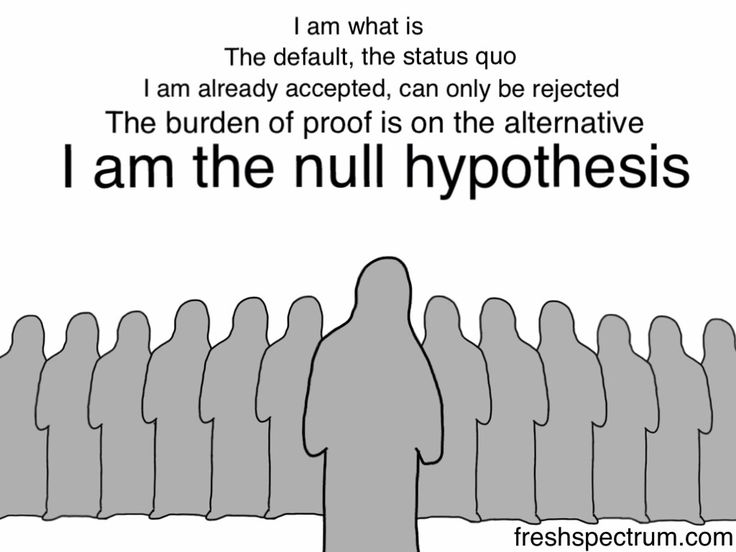
\includegraphics[width=0.5\linewidth]{nhst}
		\end{figure}
		
	\end{frame}
	
%	\begin{frame}
%		% TODO: \usepackage{graphicx} required
%		\begin{figure}
%			\centering
%			
\includegraphics[width=0.7\linewidth]{nhstYoda}
%		\end{figure}
%		
%	\end{frame}
	
	
	\begin{frame}
		\begin{enumerate}
			\setcounter{enumi}{1}
			\item \textbf{Ipotesi $H_1$}: è l’ipotesi alternativa, solitamente l’ipotesi di ricerca secondo la quale i risultati ottenuti \textbf{non sono casuali} ma sono spiegabili secondo una qualche regola o teoria.
			L'ipotesi alternativa può essere:
			\tikzstyle{na} = [baseline=-.5ex]
			
			\vspace{1.5mm}
			%	\begin{itemize}
				\Large
				\centering \textbf{Bidirezionale}:
				
				\begin{equation*}
					\tikz[baseline]{
						\node[fill=blu!20, anchor=base] (t3)
						{$	\theta \neq \theta_0$};
					}
				\end{equation*}
				
	
				\Large
				\vspace{1.5mm}
				\textbf{Monodirezionale}: 
				
				\begin{columns}[T]
					
					\begin{column}{.50\linewidth}
						\centering
						\Large
						\textbf{Sinistra}
						\begin{equation*}
							\tikz[baseline]{
								\node[fill=giallo!20, anchor=base] (t3)
								{$	\theta < \theta_0$};
							}
						\end{equation*}
					\end{column}
					
	
					\begin{column}{.50\linewidth}
						\centering
						\Large
						\textbf{Destra}
						\begin{equation*}
							\tikz[baseline]{
								\node[fill=olive!20, anchor=base] (t3)
								{$	\theta > \theta_0$};
							}
						\end{equation*}
					\end{column}
				\end{columns}
			\end{enumerate}
		\end{frame}
		
		
	
		\begin{frame}
			\begin{exampleblock}{Esempio}
				
				Si vuole stabilire, attraverso un esperimento, se una moneta sia truccata o meno. Si indicherà con $P$ la probabilità di ottenere testa in un lancio. Prima di eseguire l’esperimento si devono formulare le due ipotesi relativamente al parametro $\pi$:
				
				
				\vspace{3mm}
				\begin{itemize} 
					\item $H_0: \; \pi=.50$ la moneta non è truccata
					\vspace{3mm}
					
					\item $H_1: \; \pi \neq .50$ la moneta è truccata
				\end{itemize}	
			\end{exampleblock}
		\end{frame}
		
		\begin{frame}
			Il problema è stabilire se i risultati dell’esperimento (ad es. lanciare una moneta 30 volte) falsificano o meno l’ipotesi; 
			
			\vspace{3mm}
			I valori empirici possono considerarsi dovuti a fluttuazioni casuali intorno al valore atteso e di conseguenza non confutare $H_0$?
			
			\vspace{3mm}
			Oppure il risultato non lo consente, le fluttuazioni non sono casuali ma sistematiche e di conseguenza $H_0$ è confutata?
			
			
		\end{frame}
		
		\begin{frame}
			La decisione si basa sul calcolo di un test statistico e sulla probabilità associata al valore di tale test: 
			
			\vspace{3mm}
			\begin{block}{Test statistico}
				Valore di una variabile casuale che può assumere i valori di una distribuzione campionaria caratterizzata da una determinata distribuzione di probabilità
			\end{block}
			
			Ogni test statistico divide lo spazio campionario: 
			
			\begin{enumerate}
				\item Regione di non rifiuto di $H_0$
				\item Regione di  rifiuto di $H_0$
			\end{enumerate}
			
			In base alla regione in cui andrà a cadere il valore campionario, si prenderà una decisione sull’ipotesi $H_0$
		\end{frame}
		
		\begin{frame}
			Le regioni di rifiuto e di accettazione corrispondono ad aree di probabilità sottese alla curva
			
			\begin{figure}
				\centering
				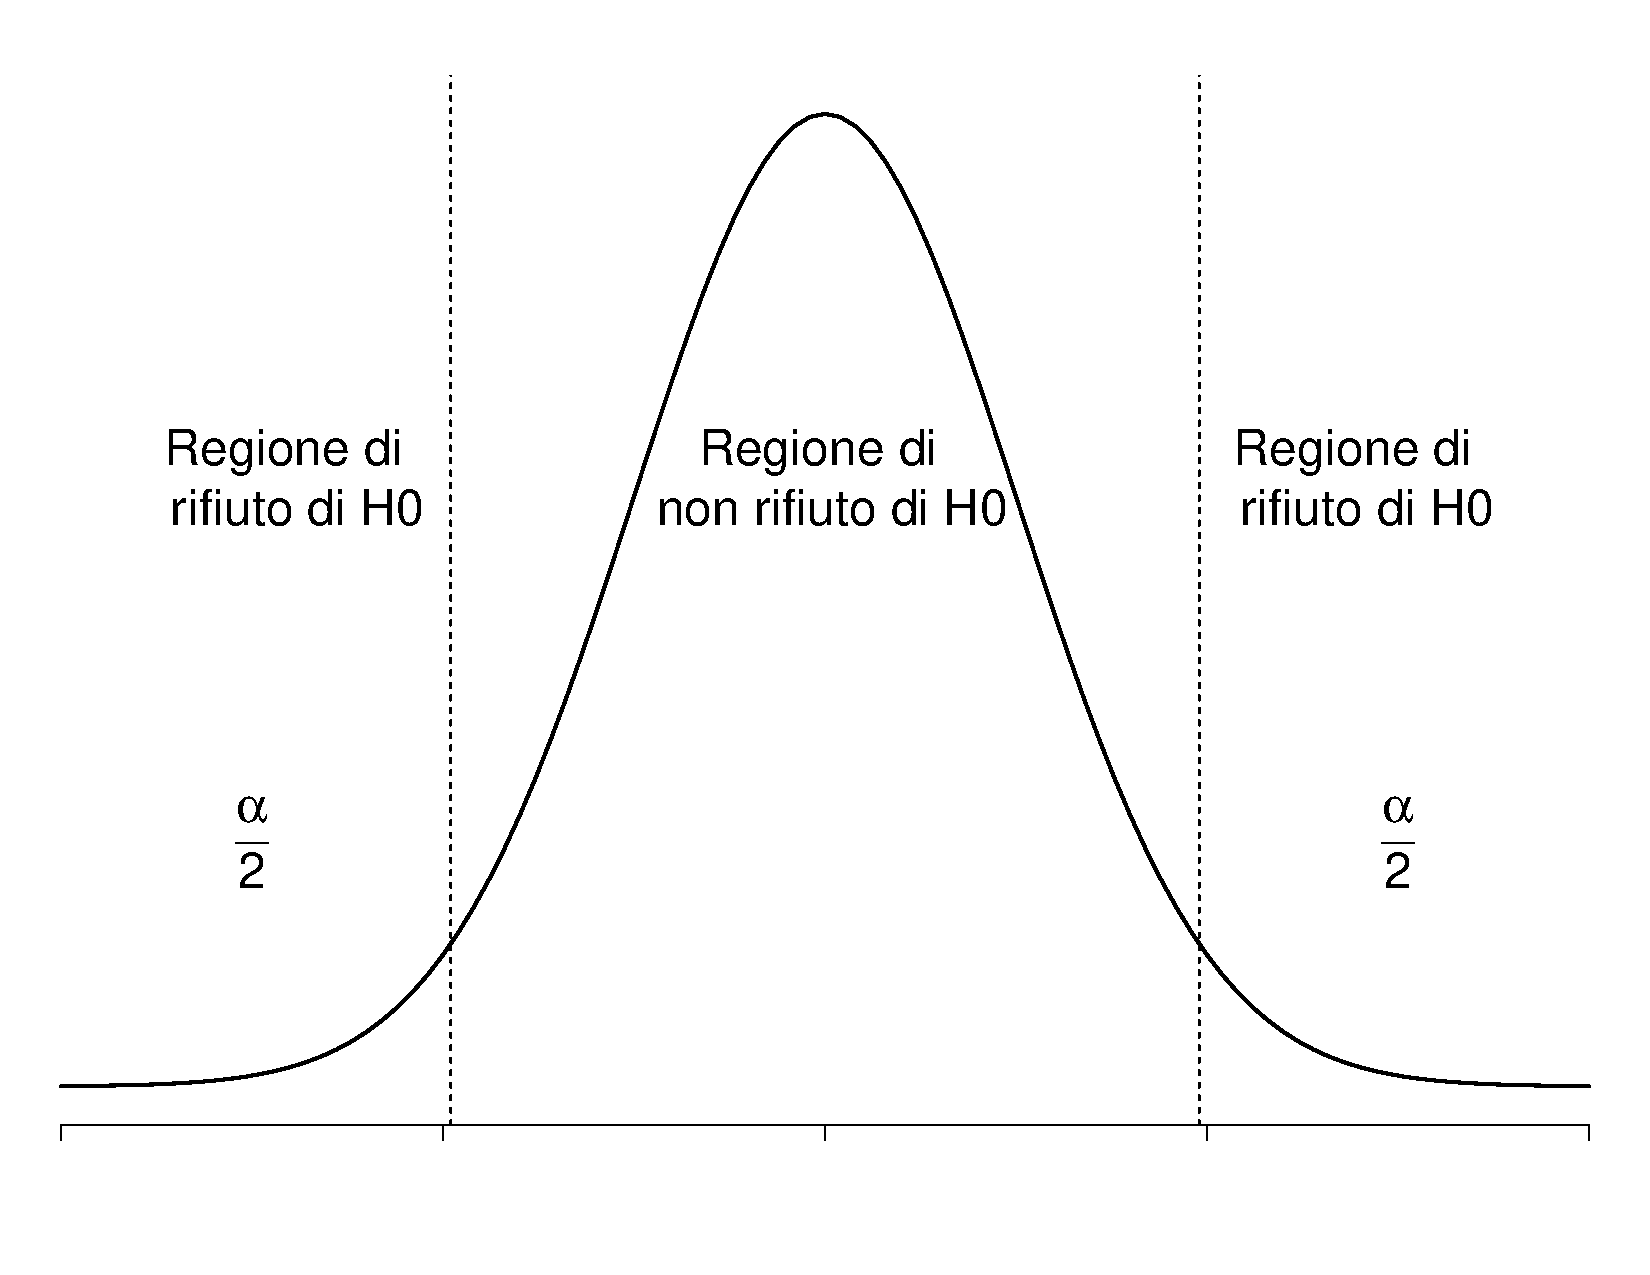
\includegraphics[width=.60\linewidth]{regioneRifiutobi.pdf}
			\end{figure}
			
			\vspace{-1.5mm}
			\begin{columns}[T]
				\column{.50\linewidth}
				\small
				\textbf{Regione di non rifiuto}: valori delle statistiche campionarie con probabilità maggiori di verificarsi
				
				\column{.50\linewidth}
				\small
				\textbf{Regione di rifiuto}: valori delle statistiche campionarie con probabilità molto basse di verificarsi
			\end{columns}
		\end{frame}
	
	\section{Distribuzioni campionarie}
	
	\begin{frame}{Distribuzione campionaria}
		
		\begin{quote}
			La \textbf{distribuzione campionaria} è la \emph{distribuzione di probabilità} relativa a una specifica statistica calcolata su tutti i $k$ campioni estraibili da una popolazione
		\end{quote}
		
		Per determinare una distribuzione campionaria: 
		
		\begin{enumerate}
			\item Estrarre tutti i possibili $k$ campioni dalla popolazione di interesse con campionamento \emph{casuale e indipendente} \color{blu} $\rightarrow$ \normalcolor ogni unità di analisi deve avere la stessa probabilità di essere estratta e l'estrazione di una unità non deve modificare la probabilità delle altre unità
			
			\item Calcolare su ognuno dei $k$ campioni la statistica di interesse
			
			\item Determinare (i.e., contare) la frequenza per ognuno dei valori della statistica \color{blu} $\rightarrow$ \normalcolor quanti \emph{campioni} presentano quel valore
		\end{enumerate}
		
	\end{frame}
	
	\subsection{Distribuzione campionaria della media}
	
%	\begin{frame}
%		Se si estraggono tutti i possibili campioni di ampiezza $n$ da una popolazione (con $\mu$ e $\sigma$) e si calcola per ognuno la media
%		
%		\vspace{3mm}
%		\begin{center}
%			
\includegraphics[width=0.06\linewidth]{frecciadown.png}
%			
%			\vspace{3mm}
%			DISTRIBUZIONE CAMPIONARIA DELLA MEDIA (\emph{d}CM)
%		\end{center}
%		
%		La distribuzione campionaria della media ha forma normale ed è caratterizzata da una media ($\mu_M$) e una deviazione standard detto \textbf{errore standard} ($\sigma_M$)
%		
%	\end{frame}
%	
	\begin{frame}
		\begin{tikzpicture}
			\node (a) [type1, xshift=-3cm] {};
			\node (b) [type2, right of=a, xshift=0.5cm]{};
			\node (c) [type3, right of=b, xshift=0.5cm]{};
			\node (d) [type4, right of=c, xshift=0.5cm]{};
			\node (e) [type5, right of=d, xshift=0.5cm]{};
			\node (f) [type6, right of=e, xshift=0.5cm]{};
			\node (pop)[info, right of =f , xshift=1.5cm] {Popolazione};
			\onslide<2->
			\node[draw=red,fit=(a) (b) ,inner sep=0.8ex,ellipse] (c1) {};
			\node[draw=black,fit=(b) (c) ,inner sep=0.5ex,ellipse] (c2) {};
			\node[draw=blue,fit=(c) (d) ,inner sep=0.8ex,ellipse] (c3) {};
			\node[draw=cyan,fit=(d) (e) ,inner sep=0.5ex,ellipse] (c4) {};	
			\node[draw=olive,fit=(e) (f) ,inner sep=0.8ex,ellipse] (c5) {};
			
			\node (g1a) [type1,below of=c1, xshift=-0.8cm, yshift=-0.5cm] {};
			\node (g1b) [type2,right of=g1a, xshift=-0.3cm] {};
			\node[draw = black, fit = (g1a) (g1b), rectangle] (g1) {};
			
			\node (g2a) [type2,right of=g1b, xshift=0.15cm] {};
			\node (g2b) [type3,right of=g2a, xshift=-0.3cm] {};
			\node[draw = black, fit = (g2a) (g2b), rectangle] (g2) {};
			
			
			\node (g3a) [type3,right of=g2b, xshift=0.15cm] {};
			\node (g3b) [type4,right of=g3a, xshift=-0.3cm] {};
			\node[draw = black, fit = (g3a) (g3b), rectangle] (g3) {};
			
			\node (g4a) [type4,right of=g3b, xshift=0.15cm] {};
			\node (g4b) [type5,right of=g4a, xshift=-0.3cm] {};
			\node[draw = black, fit = (g4a) (g4b), rectangle] (g4) {};
			
			\node (g5a) [type5,right of=g4b, xshift=0.15cm] {};
			\node (g5b) [type6,right of=g5a, xshift=-0.3cm] {};
			\node[draw = black, fit = (g5a) (g5b), rectangle] (g5) {};
			
			\node (campione) [info, right of=g5, xshift=1.5cm] {Campione};
			
			\draw[thick,->,>=stealth, red] (c1) edge  (g1);
			\draw[thick,->,>=stealth, black] (c2) edge  (g2);
			\draw[thick,->,>=stealth, blue] (c3) edge  (g3);
			\draw[thick,->,>=stealth, cyan] (c4) edge  (g4);
			\draw[thick,->,>=stealth, giallo] (c5) edge  (g5);
			\onslide<3->	
			\node (m1) [stat, below of= g1, yshift=-1cm] {\color{red}$M_1$};
			\node (m2) [stat, below of= g2, yshift=-1cm] {\color{black}$M_2$};
			\node (m3) [stat, below of= g3, yshift=-1cm] {\color{blue}$\ldots$};
			\node (m4) [stat, below of= g4, yshift=-1cm] {\color{cyan}$\ldots$};
			\node (m5) [stat, below of= g5, yshift=-1cm] {\color{giallo}$M_5$};
			
			\draw[thick,->,>=stealth] (g1) edge  (m1);
			\draw[thick,->,>=stealth] (g2) edge  (m2);
			\draw[thick,->,>=stealth] (g3) edge  (m3);
			\draw[thick,->,>=stealth] (g4) edge  (m4);
			\draw[thick,->,>=stealth] (g5) edge  (m5);
			
			\node (statistica) [info, right of= m5, xshift = 1cm] {Statistica};
			
			\onslide<4->
			\node (mediaGen) [info, below of= m3, yshift= -1cm] {$\mu_{\bar{X}} = \frac{M_1 + M_2 + \ldots + M_k}{\text{k}}$};
			\node (statistica) [info, below of= statistica,  yshift= -1cm] {Distribuzione campionaria della media};
			
			\draw[thick,->,>=stealth] (m1) edge  (mediaGen);
			\draw[thick,->,>=stealth] (m2) edge  (mediaGen);
			\draw[thick,->,>=stealth] (m3) edge  (mediaGen);
			\draw[thick,->,>=stealth] (m4) edge  (mediaGen);
			\draw[thick,->,>=stealth] (m5) edge  (mediaGen);
		\end{tikzpicture}
		
		\onslide<2->
		\begin{alertblock}{N.B.:}
			
			Sono illustrati solo alcuni dei possibili $k$ campioni 
		\end{alertblock}
	\end{frame}
	
	\begin{frame}{Esempio}
		
		Popolazione: $N = 5$ \\
		Campione: $n = 2$, Somministrato un test con punteggio 0--10
		
		\begin{columns}[T]
			\begin{column}{.50\linewidth}
				\begin{center}
					Popolazione $N = 5$
				\end{center}
				\small
				\begin{tabular}{p{3cm}p{2cm}}
					\hline
					Soggetto & Punteggio \\\hline
					Giorgio & 6 \\
					Alessandra & 8 \\
					Francesco & 10 \\
					Livio & 3 \\
					Jessica & 8 \\
					\hline
				\end{tabular}
				
				\vspace{1.3mm}
				\begin{equation*}
					\mu = \dfrac{6 + 8 + 10 + 3 + 8}{5} = 7 
				\end{equation*}
			\end{column}
			\pause
			\begin{column}{.50\linewidth}
				\begin{center}
					Campione $n = 2$
				\end{center}
				\small
				\scalebox{.65}{
					\begin{tabular}{p{3cm}p{2cm}}
						\hline
						Soggetto & Punteggio \\\hline
						Giorgio & 6 \\
						Alessandra & 8 \\
						\hline
					\end{tabular}
				}
				\begin{equation*}
					\bar{X} = \dfrac{6 + 8}{2} = 7
				\end{equation*}
				
				\pause 
				E un altro campione? 
				\scalebox{.65}{
					\begin{tabular}{p{3cm}p{2cm}}
						\hline
						Soggetto & Punteggio \\\hline
						Alessandra & 8 \\
						Francesco & 10 \\
						\hline
					\end{tabular}
				}
				
				\begin{equation*}
					\bar{X} = \dfrac{8 + 10}{2} = 9
				\end{equation*}
			\end{column}
		\end{columns}
	\end{frame}
	
\begin{frame}{Esempio}
	
	Popolazione: $N = 5$ \\
	Campione: $n = 2$, Somministrato un test con punteggio 0--10
	
	\begin{columns}[T]
		\begin{column}{.50\linewidth}
			\begin{center}
				Popolazione $N = 5$
			\end{center}
			\small
			\begin{tabular}{p{3cm}p{2cm}}
				\hline
				Soggetto & Punteggio \\\hline
				Giorgio & 6 \\
				Alessandra & 8 \\
				Francesco & 10 \\
				Livio & 3 \\
				Jessica & 8 \\
				\hline
			\end{tabular}
			
			\vspace{1.3mm}
			\begin{equation*}
				\mu = \dfrac{6 + 8 + 10 + 3 + 8}{5} = 7 
			\end{equation*}
		\end{column}
		\pause
		\begin{column}{.50\linewidth}
			\begin{center}
				Campione $n = 2$
			\end{center}
			\small
			\scalebox{.65}{
				\begin{tabular}{p{3cm}p{2cm}}
					\hline
					Soggetto & Punteggio \\\hline
					Giorgio & 6 \\
					Alessandra & 8 \\
					\hline
				\end{tabular}
			}
			\begin{equation*}
				\bar{X} = \dfrac{6 + 8}{2} = 7
			\end{equation*}
			
			\pause 
			E un altro campione? 
			\scalebox{.65}{
				\begin{tabular}{p{3cm}p{2cm}}
					\hline
					Soggetto & Punteggio \\\hline
					Alessandra & 8 \\
					Francesco & 10 \\
					\hline
				\end{tabular}
			}
			
			\begin{equation*}
				\bar{X} = \dfrac{8 + 10}{2} = 9
			\end{equation*}
		\end{column}
	\end{columns}
\end{frame}

\begin{frame}{Tutti i campioni possibili}
	\scalebox{.50}{
		\begin{tabular}{c|ccc  ca|c|c ccca}
			\hline
			Campione 	&	Elemento 1	&	Elemento 2 	&	Valore 1	&	Valore 2	&	\textbf{Media} 	&	Campione 1	&	Elemento 1	&	Elemento 2 	&	Valore 1	&	Valore 2	&	\textbf{Media} 	\\\hline
			1	&	G	&	G	&	6	&	6	&	6	&	16	&	L	&	G	&	3	&	6	&	4.5	\\
			2	&	G	&	A	&	6	&	8	&	7	&	17	&	L	&	A	&	3	&	8	&	5.5	\\
			3	&	G	&	F	&	6	&	10	&	8	&	18	&	L	&	F	&	3	&	10	&	6.5	\\
			4	&	G	&	L	&	6	&	3	&	4.5	&	19	&	L	&	L	&	3	&	3	&	3	\\
			5	&	G	&	J	&	6	&	8	&	7	&	20	&	L	&	J	&	3	&	8	&	5.5	\\
			6	&	A	&	G	&	8	&	6	&	7	&	21	&	J	&	G	&	8	&	6	&	7	\\
			7	&	A	&	A	&	8	&	8	&	8	&	22	&	J	&	A	&	8	&	8	&	8	\\
			8	&	A	&	F	&	8	&	10	&	9	&	23	&	J	&	F	&	8	&	10	&	9	\\
			9	&	A	&	L	&	8	&	3	&	5.5	&	24	&	J	&	L	&	8	&	3	&	5.5	\\
			10	&	A	&	J	&	8	&	8	&	8	&	25	&	J	&	J	&	8	&	8	&	8	\\
			11	&	F	&	G	&	10	&	6	&	8	&		&		&		&		&		&		\\
			12	&	F	&	A	&	10	&	8	&	9	&		&		&		&		&		&		\\
			13	&	F	&	F	&	10	&	10	&	10	&		&		&		&		&		&		\\
			14	&	F	&	L	&	10	&	3	&	6.5	&		&		&		&		&		&		\\
			15	&	F	&	J	&	10	&	8	&	9	&		&		&		&		&		&		\\
			\hline
			
		\end{tabular}
	}
	\footnotesize
	\begin{equation*}
		\mu_{\bar{x}} = \dfrac{6 \cdot 1 + 7 \cdot 4 + 8 \cdot 6 + 4.5 \cdot 2 + \cdot 9 \cdot 4 + 5.5 \cdot 4 + 10 \cdot 1 + 6.5 \cdot 2 + 3 \cdot 1}{25} = 7
	\end{equation*}
	
	\pause
	\begin{equation*}
		\mu = \mu_{\bar{x}} = 7
	\end{equation*}
	
\end{frame}



%\begin{frame}
%	I singoli elementi che costituiscono la DISTRIBUZIONE CAMPIONARIA DELLA MEDIA sono quindi le medie calcolate su campioni di ampiezza $n$ estratti da una popolazione
%	
%	La media della \emph{d}CM coincide con la media della popolazione
%	%
%	\begin{equation*}
%		\mu_{\bar{x}} = \mu
%	\end{equation*}
%	
%	\centering
%	
\includegraphics[width=0.04\linewidth]{frecciadown.png}
%	
%	Stimatore corretto o non distorto: La media dello stimatore deve coincidere con il parametro
%\end{frame}	
	
		\section{Valore critico}
		
		\begin{frame}
			
			\`E il valore che separa le due regioni 
			
			\vspace{1.5mm}
			Per stabilire se il valore di un test è coerente o meno con l’ipotesi nulla è necessario verificare che il suo valore sia compreso all’interno della \textbf{regione di non rifiuto}.
			
			\vspace{1.5mm}
			Se il valore campionario cade nella \textbf{regione di rifiuto} c’è da ritenere che le osservazioni campionarie si discostino dai valori più probabili della distribuzione; in tal caso si può decidere di rifiutare $H_0$.
			
			
			\begin{figure}
				\centering
				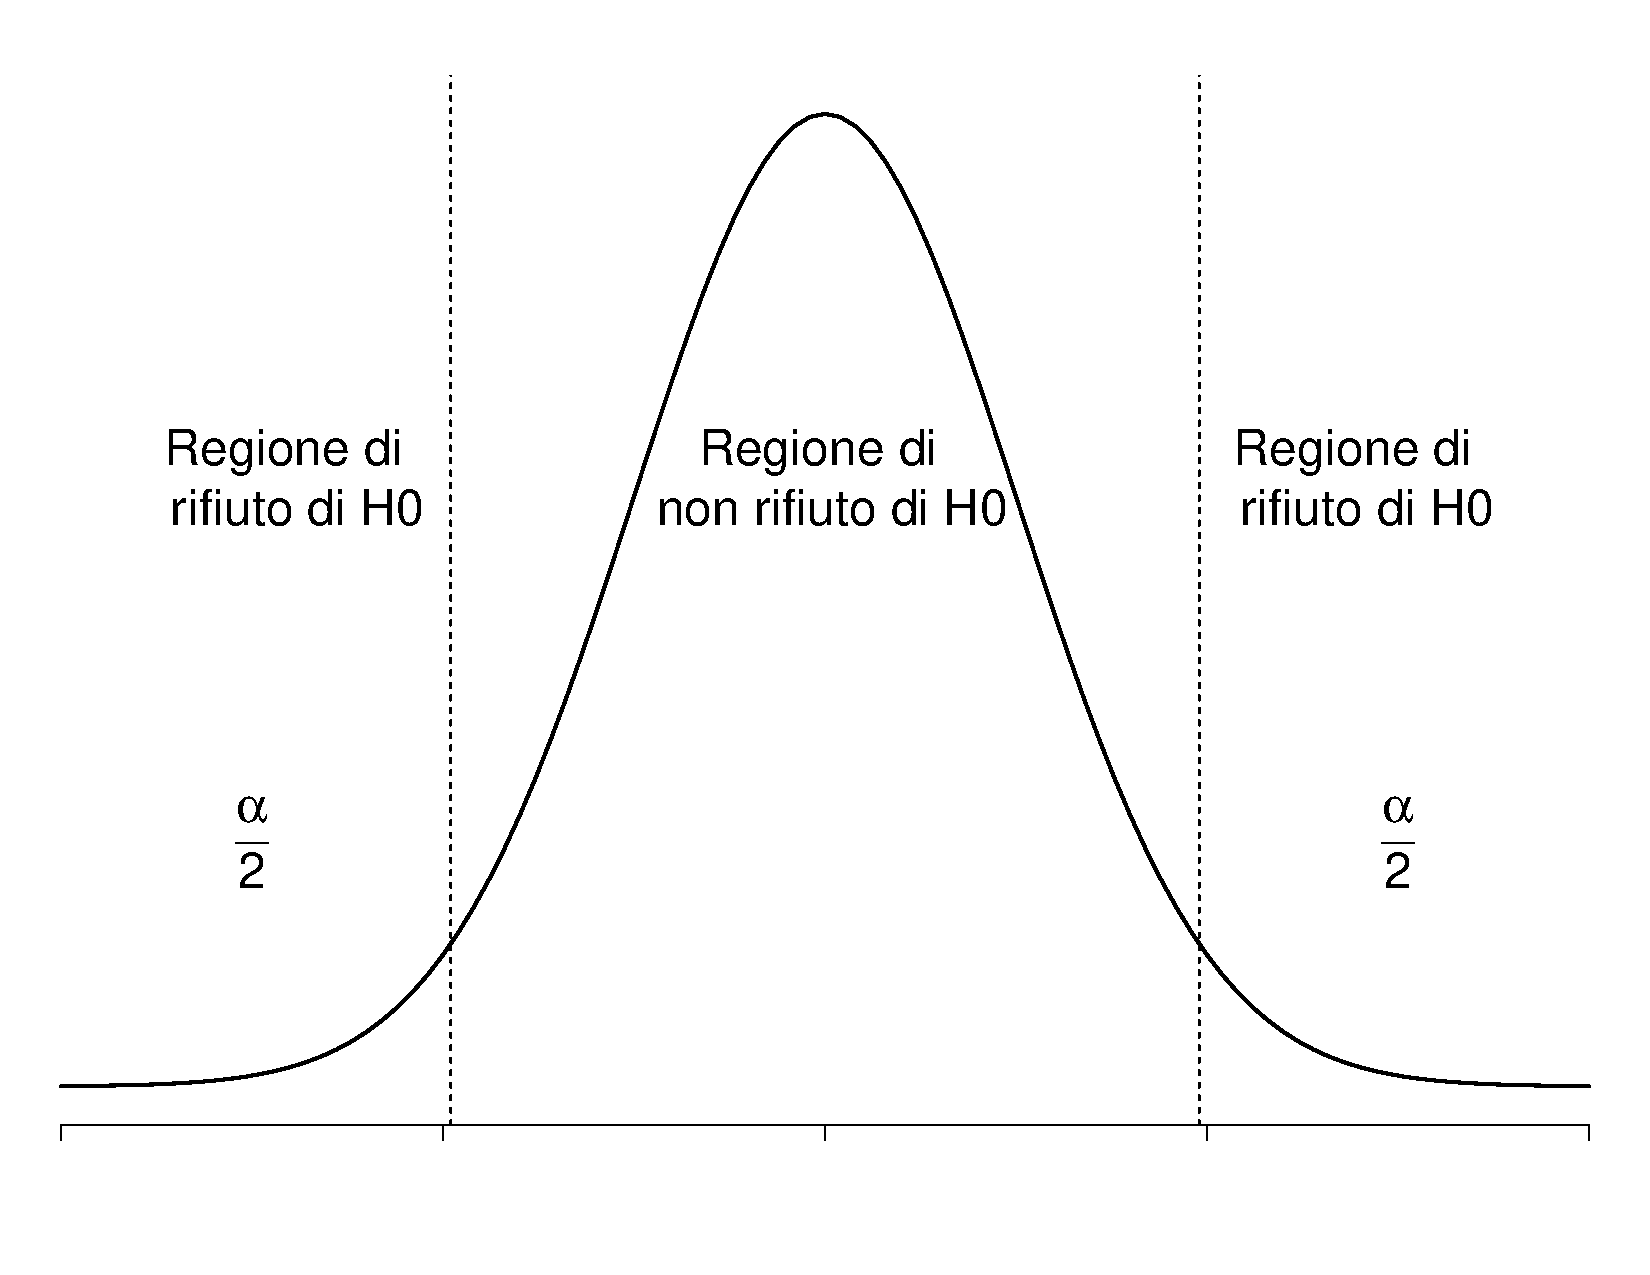
\includegraphics[width=.50\linewidth]{regioneRifiutobi.pdf}
			\end{figure}
			
		\end{frame}
		
		\begin{frame}
			
			I valori delle statistiche campionarie che cadono nella \textbf{zona di rifiuto} sono comunque in grado di verificare l’ipotesi nulla ma la loro probabilità è così bassa ($\leq \alpha$) che si accetta il rischio di rifiutare $H_0$
			
			\begin{figure}
				\centering
				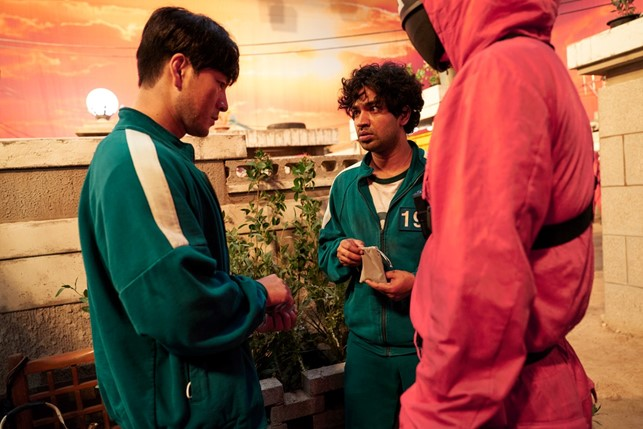
\includegraphics[width=0.6\linewidth]{attachments/squidgame}
				\caption{Stai barando vero? Come è possibile che tu vinca a ogni mano?? Le probabilità sono 50-50, vuol dire che stai barando!!!!!}
			\end{figure}
			
		\end{frame}
		
		\begin{frame}
			
			Una decisione di questo tipo comporta quindi degli errori
			
			\begin{spacing}\Factor
				\begin{tabular}{c  c  |c| c|}
					& \multicolumn{1}{c}{} & \multicolumn{2}{c}{\textcolor{blue}{Ipotesi}} \\
					& \multicolumn{1}{c}{} & \multicolumn{1}{c}{$H_0$ vera} & \multicolumn{1}{c}{$H_0$ falsa} \\
					\cline{3-4}
					\multirow{2}{*}{\textcolor{blue}{Decisione}}& Non si rifiuta $H_0$ & \textcolor{green!10!black!80}{Corretta} &  \textcolor{red}{Errata} \\
					\cline{3-4}
					& Si rifiuta $H_0$  &\textcolor{red}{Errata} &  \textcolor{green!10!black!80}{Corretta} \\
					\cline{3-4} 
				\end{tabular}
			\end{spacing}
			
			
		\end{frame}
		
		\subsection{Errori di I e II tipo}
		
		\begin{frame}
			\begin{columns}[T]
				\begin{column}{.50\linewidth}
					
					
					\begin{figure}
						\centering
						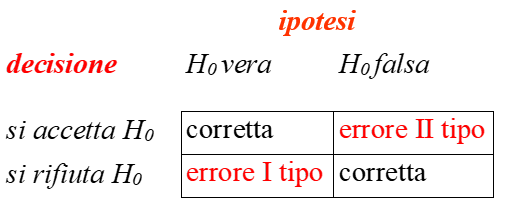
\includegraphics[width=\linewidth]{Errori.png}
					\end{figure}
				\end{column}
				\begin{column}{.50\linewidth}
					\begin{figure}
						\centering
						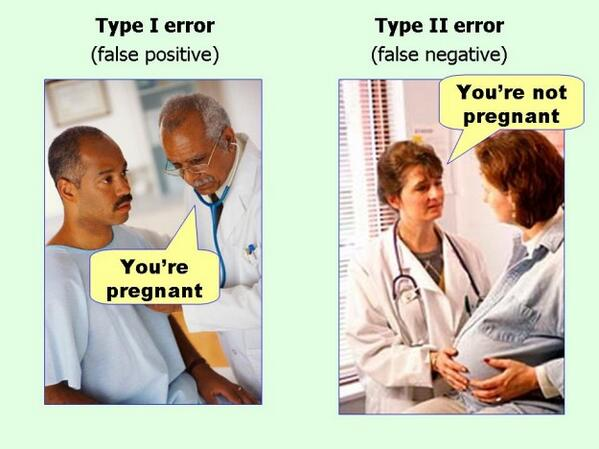
\includegraphics[width=
						\linewidth]{pregnant.jpg}
					\end{figure}
				\end{column}
			\end{columns}
			
			
			\vspace{3mm}
			
			Non è mai possibile sapere con certezza se è vera $H_0$, l’unica cosa che si può fare è \textbf{minimizzare} la probabilità di prendere una decisione sbagliata
			
			
		\end{frame}
		
		\begin{frame}
			Si è definita la probabilità di non rifiutare $H_0$ quando è vera come $1-\alpha$
			
			
			Facendo un ragionamento analogo su $H_1$ e definendo $\beta$ la probabilità di non rifiutare $H_0$ quando è falsa si avrà una regione $1- \beta$ che corrisponde alla probabilità di rifiutare $H_0$ quando è falsa
			
			\begin{spacing}\Factor
				\begin{tabular}{c  c  |c| c|}
					& \multicolumn{1}{c}{} & \multicolumn{2}{c}{\textcolor{blue}{Ipotesi}} \\
					& \multicolumn{1}{c}{} & \multicolumn{1}{c}{$H_0$ vera} & \multicolumn{1}{c}{$H_0$ falsa} \\
					\cline{3-4}
					\multirow{2}{*}{\textcolor{blue}{Decisione}}& Non si rifiuta $H_0$ & \textcolor{green!10!black!80}{Corretta} ($1-\alpha$)&  \textcolor{red}{Errore di II tipo} ($\beta$ )\\
					\cline{3-4}
					& Si rifiuta $H_0$  &\textcolor{red}{Errore di I tipo} ($\alpha$) &  \textcolor{green!10!black!80}{Corretta} ($1-\beta$)\\
					\cline{3-4} 
				\end{tabular}
			\end{spacing}
	\vspace{3mm}
	
	Quello che si controlla: $\alpha$ (la probabilità di commettere un errore di I tipo)
	
	Quello che viene ignorato: $\beta$ (la probabilità di commettere un errore di II tipo)	
			
		\end{frame}
		
		
		\begin{frame}{Relazione tra $\alpha$ e $\beta$}
			
			   \begin{tikzpicture}[remember picture, overlay]
				\node[anchor=north east, yshift=-0.5cm, xshift=-2cm] at (current page.north east) {
					\footnotesize
					\begin{tabular}{ccc}
						\hline
						$\alpha$ & $\beta$ & $1 - \beta$ \\ \hline
						.10 & .04 & .96\\ 
						.05 & 0.09 & .91 \\ 
						.01 & 0.25 & .75 \\ 
						.001& 0.54 & .46 \\\hline
					\end{tabular}
				};
			\end{tikzpicture}
			
			\begin{figure}
					\centering
				\begin{subfigure}{.4\linewidth}
					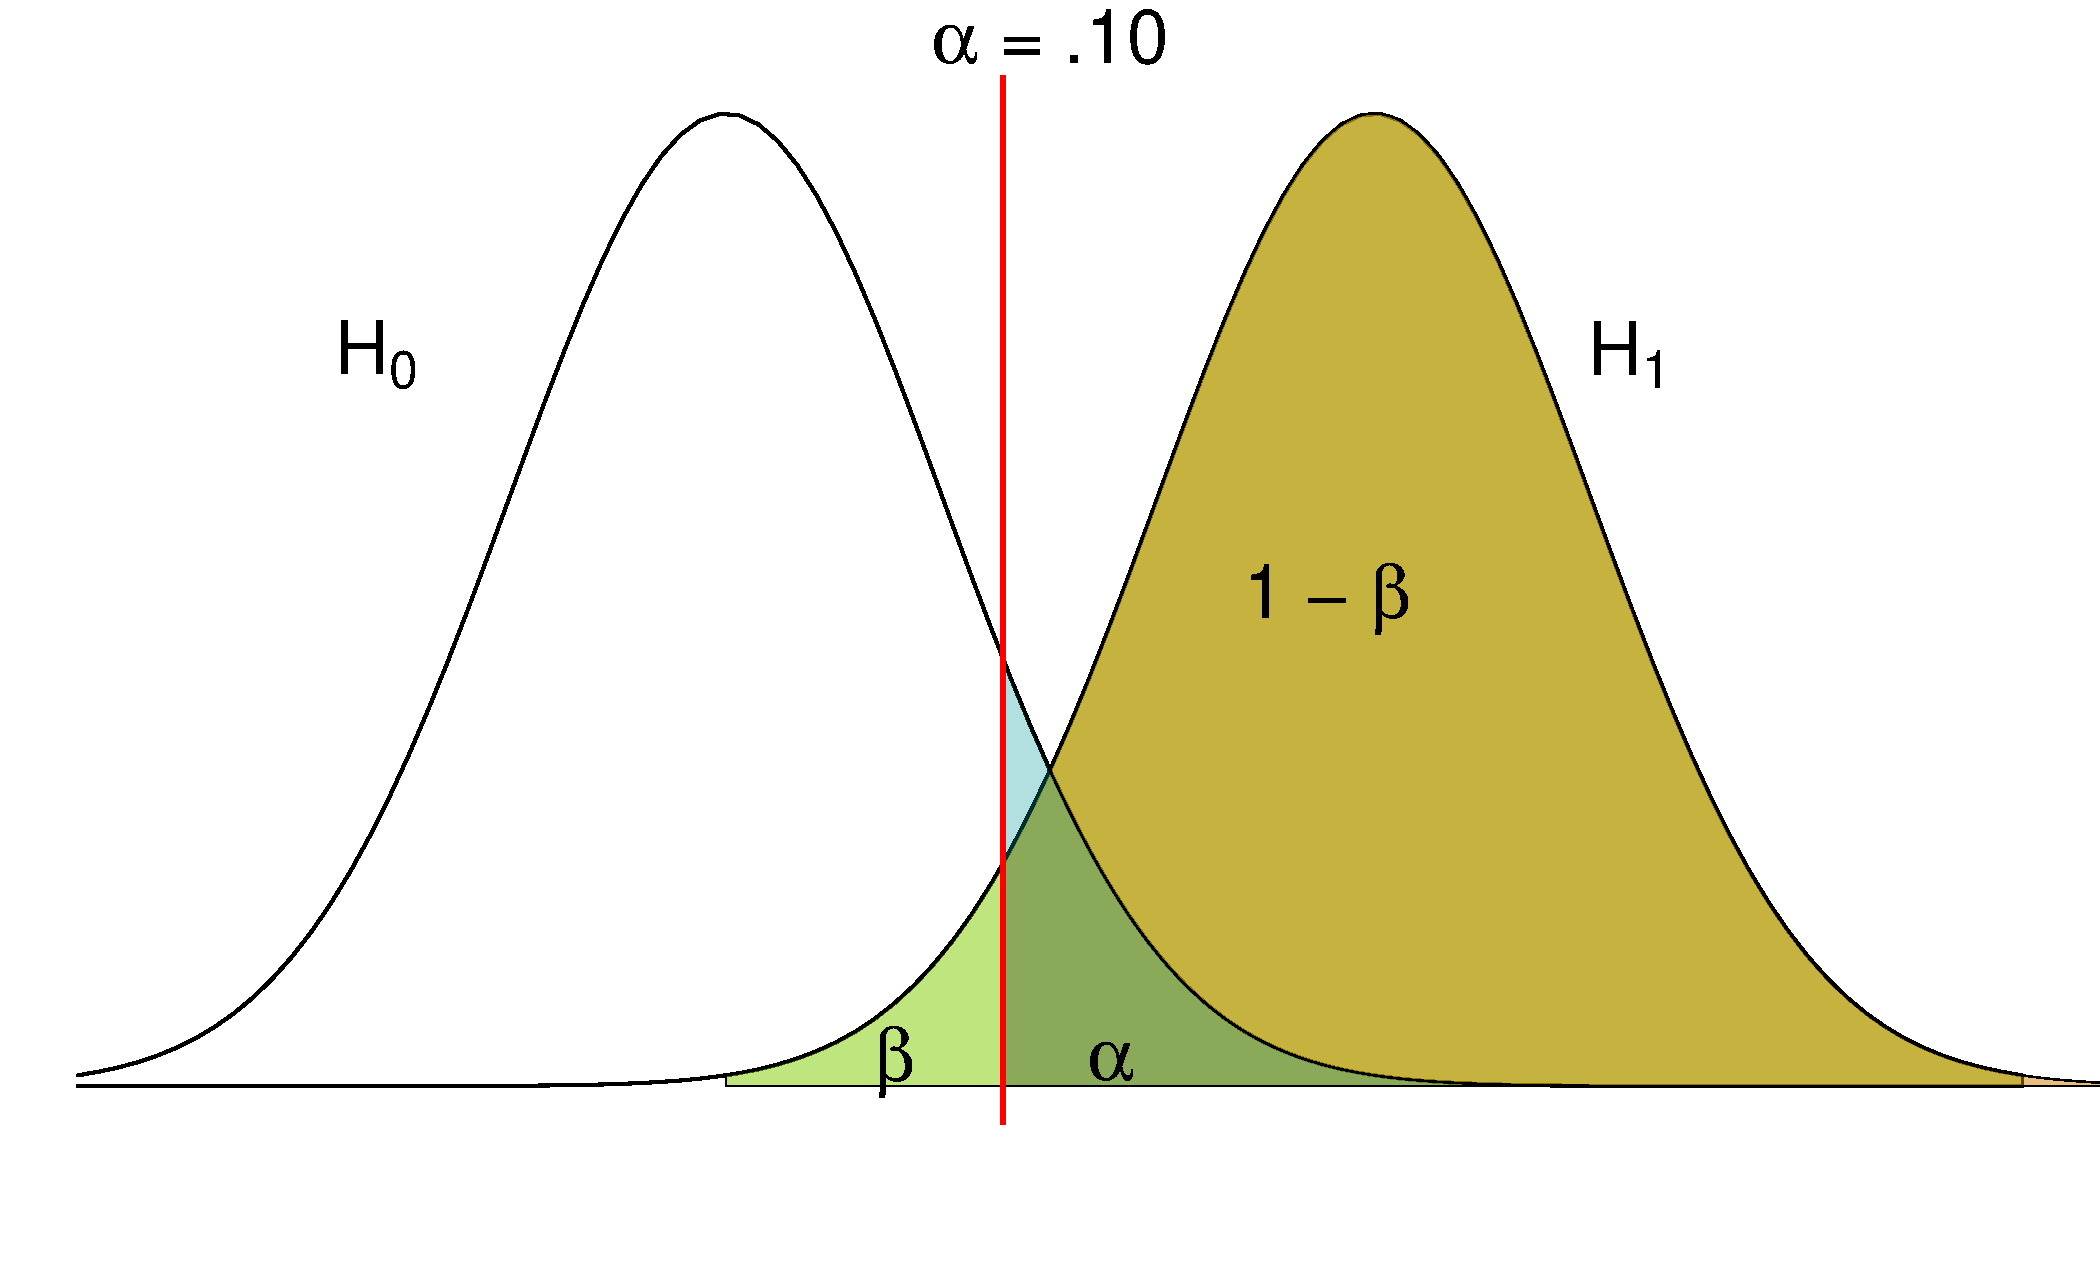
\includegraphics[width=\linewidth]{img/power10}
				\end{subfigure}
				\begin{subfigure}{.4\linewidth}
					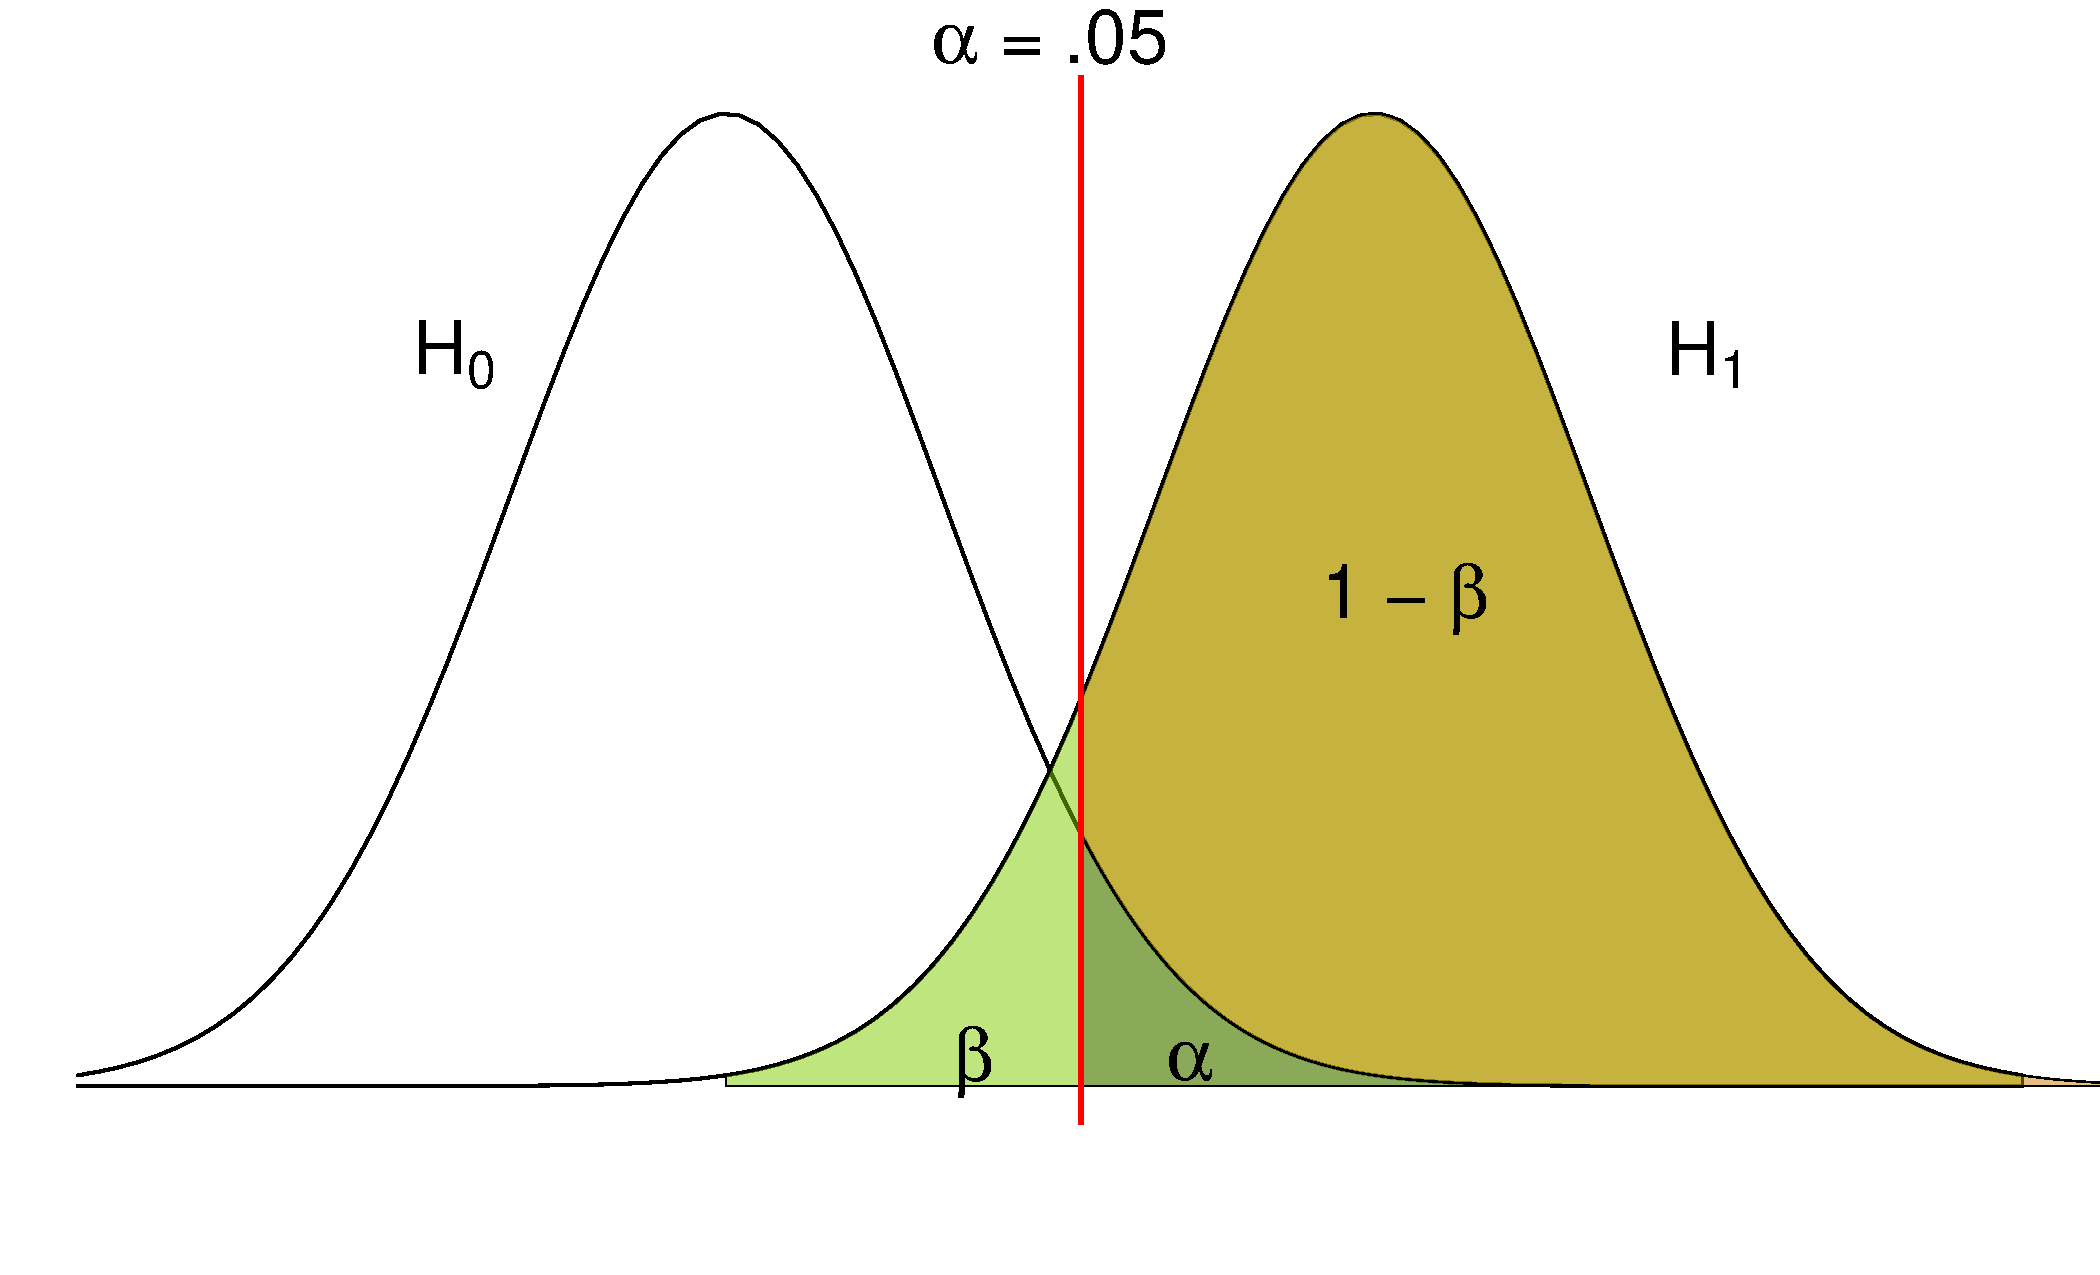
\includegraphics[width=\linewidth]{img/power05}
				\end{subfigure}
				
				\begin{subfigure}{.4\linewidth}
					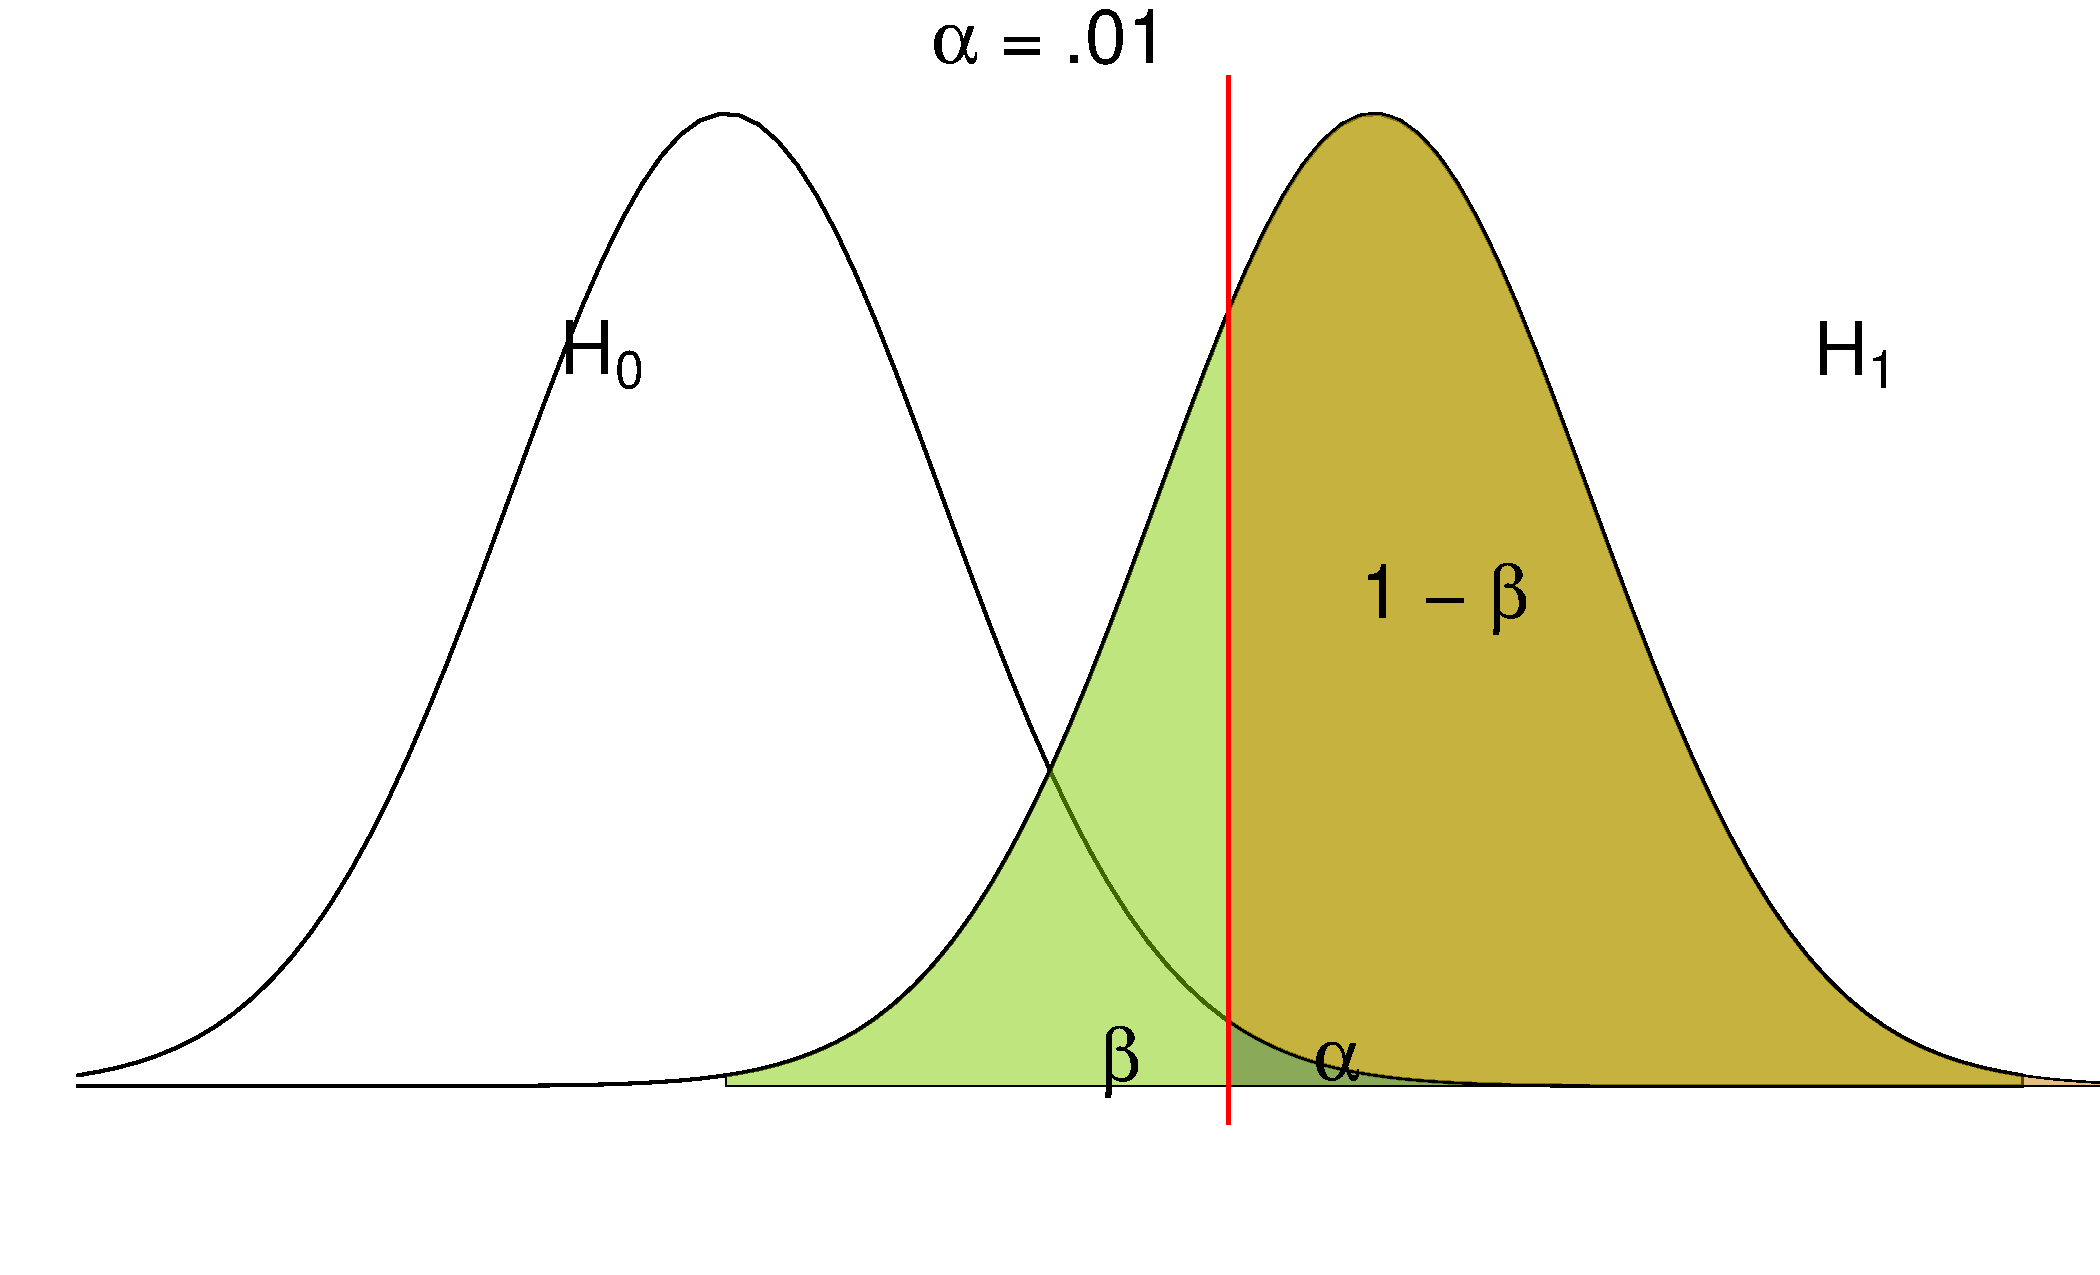
\includegraphics[width=\linewidth]{img/power01}
				\end{subfigure}
				\begin{subfigure}{.4\linewidth}
					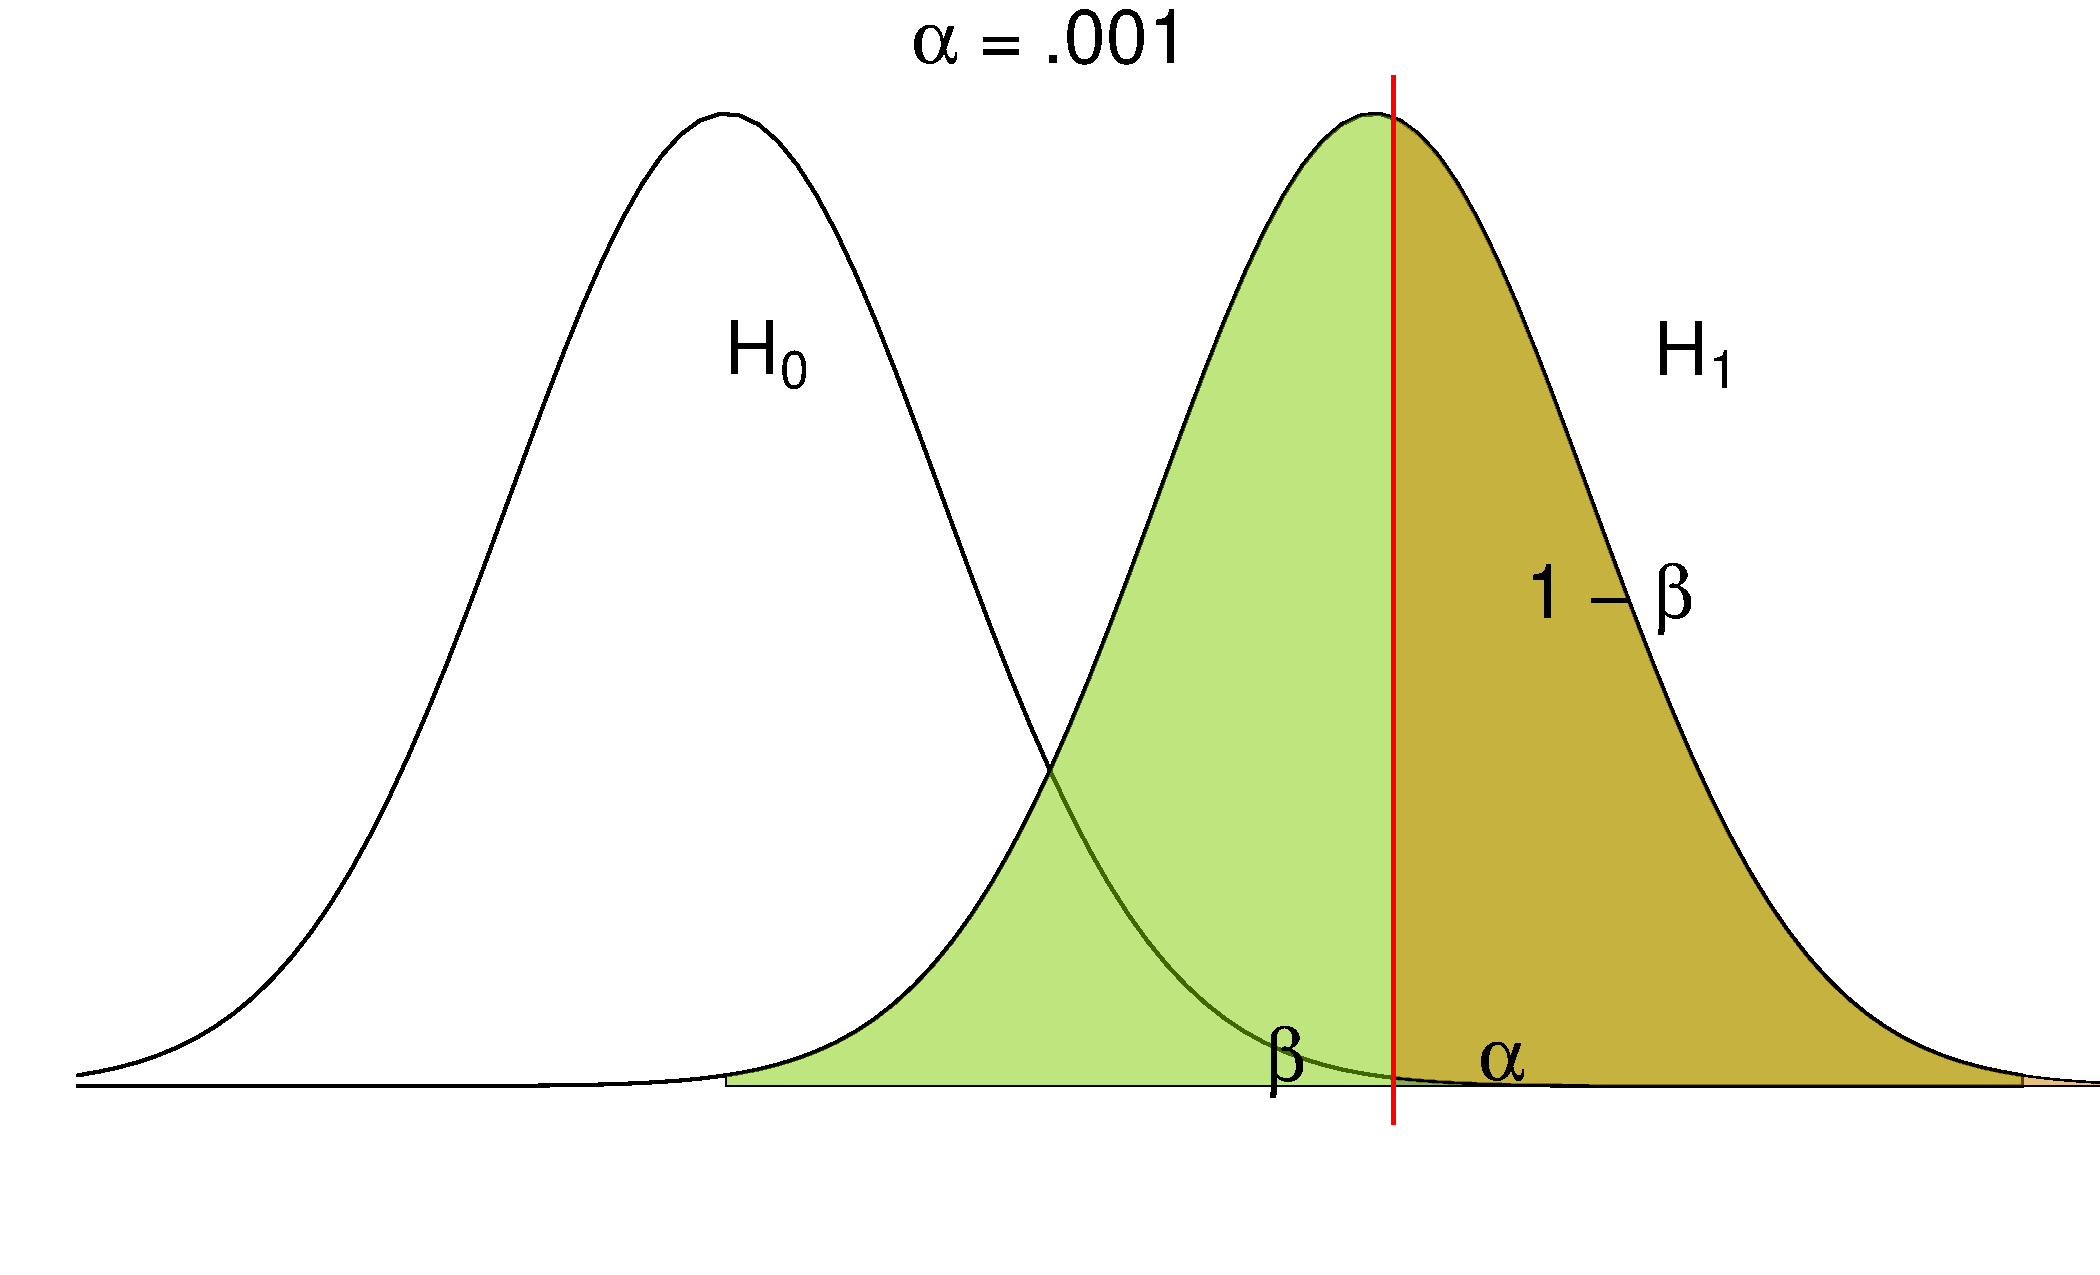
\includegraphics[width=\linewidth]{img/power001}
				\end{subfigure}
			\end{figure}
		
	  $\mu_0 = 0$, $\mu_1 = 3$
		\end{frame}

\subsection{Regola Decisionale}
\begin{frame}
	\small
	\begin{block}{}
		In generale, se indichiamo con $\psi_c$ e $\psi_o$ rispettivamente il \textbf{valore critico} e il \textbf{valore osservato} di una statistica $\psi$, allora sussiste il seguente rapporto relazionale tra $(p\text{-value}, \alpha)$ e $(\psi_c, \psi_o)$:
	\end{block}
	
	\vspace{0.3cm}
	
	\begin{columns}[T]
		\column{0.45\textwidth}
		\centering
		\fbox{
			\begin{minipage}{0.85\textwidth}
				\[
				\begin{aligned}
					p\text{-value} &< \alpha \Rightarrow H_A \\
					p\text{-value} &\geq \alpha \Rightarrow \neg H_A
				\end{aligned}
				\]
			\end{minipage}
		}
		
		\column{0.1\textwidth}
		\vspace*{5mm}
		\centering
		\Large $\Leftrightarrow$
		
		\column{0.45\textwidth}
		\centering
		\fbox{
			\begin{minipage}{0.85\textwidth}
				\[
				\begin{aligned}
					\psi_c &< \psi_o \Rightarrow H_A \\
					\psi_c &\geq \psi_o \Rightarrow \neg H_A
				\end{aligned}
				\]
			\end{minipage}
		}
	\end{columns}
	
	\vspace{0.5cm}
	
	\setbeamercolor{block body}{bg=black!70,fg=yellow}
	\begin{block}{}
		\textbf{Un risultato si dice \underline{statisticamente significativo}} (rigetto ipotesi nulla $H_0$) nel caso in cui il valore della statistica critica $\psi_c$ (calcolato sulla base di $\alpha$) sia strettamente minore del valore della statistica osservata $\psi_o$. \\[6pt]
		\textbf{Un risultato si dice \underline{statisticamente non significativo}} (non rigetto ipotesi nulla $H_0$) nel caso in cui il valore della statistica critica $\psi_c$ (calcolato sulla base di $\alpha$) sia maggiore o uguale al valore della statistica osservata $\psi_o$.
	\end{block}
	
\end{frame}

%\begin{frame}{Regola decisionale}
%	
%	\begin{block}{$T_0$ vs. $T_{\text{critico}}$}
%		
%		Si confronta il valore della statistica $T_0$ con il valore critico $T_{\text{critico}}$ stabilito sulla base di $\alpha$, del tipo di ipotesi alternativa, dell'ampiezza campionaria, dei parametri noti della popolazione
%		
%		$|T_0| > |T_{\text{critico}}|$: Si rifiuta $H_0$
%		
%		$|T_0| < |T_{\text{critico}}|$: Non si rifiuta $H_0$
%	\end{block}
%	
%	\begin{block}{$p$-value}
%	
%	Viene calcolata la probabilità associata a $T_0$: 
%	
%	$p$-value $< \alpha$: Si rifiuta $H_0$
%	
%	$p$-value $> \alpha$: Non si rifiuta $H_0$
%	\end{block}
%\end{frame}
		
\subsection{Cos'è il $p$-value?}		
\begin{frame}
	
\begin{center}
	\emph{Il p-value indica la probabilità di osservare un valore uguale o più estremo rispetto a quello osservato, \textbf{posto che sia vera $H_0$}}
	
	$P(x \geq T_0|H_0) = p\text{-value}$
\end{center}


\begin{exampleblock}{Un esempio}
	
	$T_0 = 2.70$, $p$-value = $.0073$ ($p < .001$)
	 
	 Replicando per molte molte volte l'esperimento, quante volte ci si aspetta di rifiutare $H_0$? 
	 
	 \pause
	 
	 $P(T_0 \geq 2.70|H_0) = .0073$: Se fosse vera $H_0$, il risultato osservato sarebbe un risultato estremamente poco probabile, per cui questo risultato si osserverebbe meno dell'1\% delle volte
\end{exampleblock}

\end{frame}	

\begin{frame}{Dettagli sul $p$-value}
	
	\begin{itemize}
		\item Il $p$-value è la probabilità di ottenere un valore uguale o più estremo rispetto a $T_0$ \emph{se $H_0$ fosse vera}. \underline{NON} è la probabilità che $H_0$ sia vera $\rightarrow$ non può essere usato come indicatore della verità o falsità di $H_0$
		\item Il $p$-value è sensibile all'ampiezza campionaria: All'aumentare dell'ampiezza campionaria, diminuisce il $p$-value, aumenta la probabilità di rigettare $H_0$
		\item Il $p$-value permette solo di prendere una decisione qualitativa nei termini di ``Non rigetto $H_0$'' vs. ``Rigetto $H_0$'' $\rightarrow$ \textbf{Non è una misura dell'evidenza statistica}
		 
	\end{itemize}
\end{frame}

	
\end{document}